\chapter{Discussion}
\label{ch:futurework}


In this chapter, we discuss the findings and limitations of our project, as well as propose some future work to improve
the platform exchange and the tokens.


\section{ERC777 token standard, an alternative solution to ERC20}


In this project, the solution implemented is based on the ERC20 token standard. One alternative solution to the ERC20 token
is the ERC777 token standard proposed by Jacques Dafflon, Jordi Baylina, and Thomas Shababi \cite{erc777}. ERC777 is an advanced
token standard that addresses specific limitations encountered in our platform exchange of two tokens. While the ERC20
token standard is widely adopted and supported by most token-based systems, there are certain limitations that can
impact the efficiency and flexibility of our platform.


The ERC777 token standard introduces a more intuitive and efficient way to transfer tokens. It uses the
\texttt{send} function, similar to the \texttt{transfer} function in the ERC20 token standard, but it facilitates
users to understand and interact with the token contract. This transfer function can improve our platform exchange by
allowing users to transfer tokens without worrying about the \texttt{approve} and \texttt{transferFrom} functions.
Indeed, for example, if the recipient is a contract, users must first call the \texttt{approve} function, then the
\texttt{transferFrom} function mechanism to transfer tokens. If a user forgets and only calls the \texttt{transfer}, the
tokens will get stuck in the contract, and the user will not be able to retrieve them. There is no way to regain the tokens, and the user will lose them.


The ERC777 token standard also allows contracts and regular addresses to control or reject the tokens they
send and receive. Using the \texttt{tokenToSend} and \texttt{tokensReceived} hooks, we can implement custom logic
to validate and manage tokens transfer. These features can be helpful by providing more control and flexibility
to our platform exchange. In addition, it ensures that only authorized and verified transactions are processed on our platform.


Finally, the ERC777 token standard also introduces one significant advantage over the ERC20 token standard: the ability to
send tokens to a contract and notify the contract in a single transaction with the \texttt{tokensReceived} hook. This
feature removes a two-step process like the \texttt{approve/transferFrom} required by the ERC20 token standard, making
interaction with contracts more straightforward and efficient. In addition, this feature can be helpful by simplifying the interaction
of our platform with external contracts, such as liquidity providers.


While the ERC777 token standard offers some different features and advantages over the ERC20 token standard, its
adoption requires significant effort and time. We need to assess the impact of this change on our platform by assessing
the compatibility and readiness of existing wallets and infrastructure to support the ERC777 token standard. Moreover,
we need to update our platform to support the ERC777 token standard by updating the smart contracts and the front-end
to accommodate the new features and functionalities.

\section{Future Work: Liquidity and Automated Pricing}


One of the main limitations of our platform exchange order book is the need for more liquidity functionality. Indeed, our
exchange operates based on fixed prices and quantities for exchanging tokens. This means that users can only accept the
price and quantity offered by the other counterparty. This can be a limitation for our platform, as it can discourage
users from using it. However, a more dynamic and efficient solution would be to implement a liquidity
mechanism that automatically determines the price of a token based on the market demand and supply\footnote{The market
demand and supply is the total quantity of a token that users are willing to buy or sell at a given price.} against another
token. In traditional centralized exchanges, liquidity is often provided by market makers or specialized firms that
provide liquidity to the exchange. However, in decentralized exchanges and platforms like ours, creating liquidity is
more challenging, as there is no central authority to provide liquidity, and thus, it requires a different approach.

\begin{figure}[ht]
    \centering
    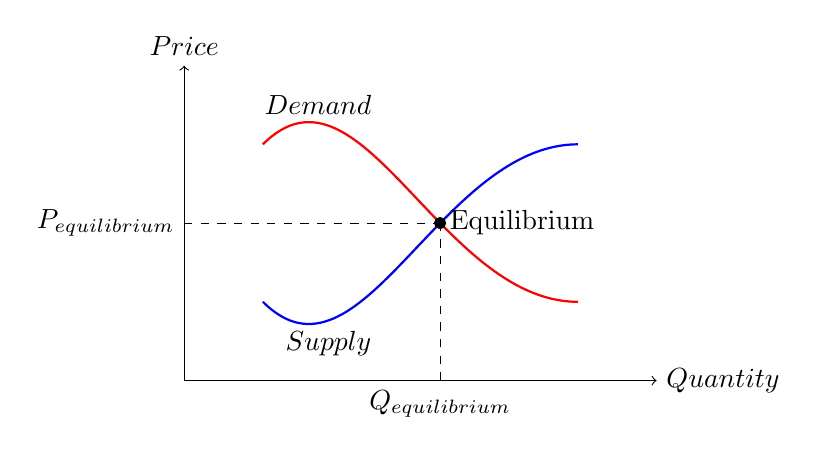
\begin{tikzpicture}
        % Axes
        \draw[->] (0,0) -- (6,0) node[right] {$Quantity$};
        \draw[->] (0,0) -- (0,4) node[above] {$Price$};

        % Supply curve
        \draw[blue, thick] (1,1) to[out=-45, in=180] (5,3);
        % \draw[dashed] (0,1) node[left] {$P_{min}$} -- (1,1);
        % \draw[dashed] (0,3) node[left] {$P_{max}$} -- (5,3);

        % Demand curve
        \draw[red, thick] (1,3) to[out=45, in=180] (5,1);

        % Equilibrium point
        \filldraw[black] (3.25,2) circle (2pt) node[right] {Equilibrium};

        % Annotations
        \draw[dashed] (3.25,0) node[below] {$Q_{equilibrium}$} -- (3.25,2);
        \draw[dashed] (0,2) node[left] {$P_{equilibrium}$} -- (3.25,2);

        % Labels
        \draw (2.5,0.75) node[below left] {$Supply$};
        \draw (2.5,3.25) node[above left] {$Demand$};

    \end{tikzpicture}

    \caption{Supply and demand curves for computing the equilibrium point.}
    \label{fig:liquidity}
\end{figure}

In figure \ref{fig:liquidity}, we illustrate that the equilibrium point between the supply and demand curves
is at the intersection of the two curves. In our platform exchange, the supply of our UET token is initially set
at its creation using the \texttt{initialSupply} parameter. This represents the total quantity of UET tokens available in the market.
However, the demand for the token is determined by the interaction of users within the liquidity pool. A liquidity pool is a
mechanism that enables users to provide liquidity by depositing their tokens into a smart contract.


Therefore, a possible solution to implement liquidity in our platform exchange is to create a liquidity pool. This smart contract holds a certain amount of our UET token and the other token. Traders can trade between these tokens
by depositing them into the liquidity pool. On the other hand, liquidity providers supply the pool with their tokens
and receive a portion of the transaction fees as a reward. These liquidity pools represent the share of the provider in
the pool.


To have a better understanding of how liquidity pools work, we can take the example of using a liquidity provider
like Uniswap \cite{uniswap}. Uniswap is a decentralized exchange protocol that allows users to swap between any two
ERC20 tokens. Users create liquidity pools for various token pairs. To illustrate, we can create a liquidity pool for
our UET token against another, such as USD Coin (USDC). To do so, we need to deposit an equal value of UET tokens and
USDC tokens into the liquidity pool. In return, we receive a liquidity pool token representing our share in the
pool.


Once the liquidity pool is created, traders can then trade between UET tokens against USDC by interacting with the
liquidity pool smart contract. Therefore, the pricing of the tokens is determined automatically within the liquidity pool
based on a constant product formula, defined by Uniswap \cite{uniswap_formula} as follows: 

\begin{equation}
    x * y = k
\end{equation}

Where $x$ and $y$ are the quantities of the tokens in the liquidity pool, and $k$ is a constant value. This formula considers the ratio of token balances in the liquidity pool. The automated pricing mechanism ensures the liquidity pool is always balanced by maintaining a balanced value between the two tokens for each trade.

By using a service like Uniswap or implementing our own liquidity pool mechanism, we can provide our platform
exchange with a more dynamic and efficient solution for trading tokens for users. It allows users to trade with a seamless
experience and access a large liquidity pool for various token pairs, e.g., UET/USDC, UET/ETH, UET/DAI, etc. Moreover,
liquidity providers can earn a portion of the transaction fees as a reward based on the trading volume in the pool,
which can incentivize them to supply liquidity and contribute to the growth of our platform exchange.

Establishing a liquidity pool mechanism requires significant careful planning and design. We need to assess
factors, such as the initial supply of the tokens and incentives for liquidity providers, and we need to especially find
a solution to attract traders to our platform exchange, which is crucial for the success of the liquidity pool.
Furthermore, the integration with other decentralized exchanges and protocols can be a challenge, as it requires
a significant effort and time to implement and test the integration.